\section{Neural network architecture}
\subsection{U-Net architecture}
The standard architecture for image segmentation tasks in the medical imaging field is the U-Net \cite{ronneberger2015u}.

Figure \ref{unet} shows the architecture of the U-Net. The left side is called the encoder, the right side the decoder.

\begin{figure}[H]
\centering
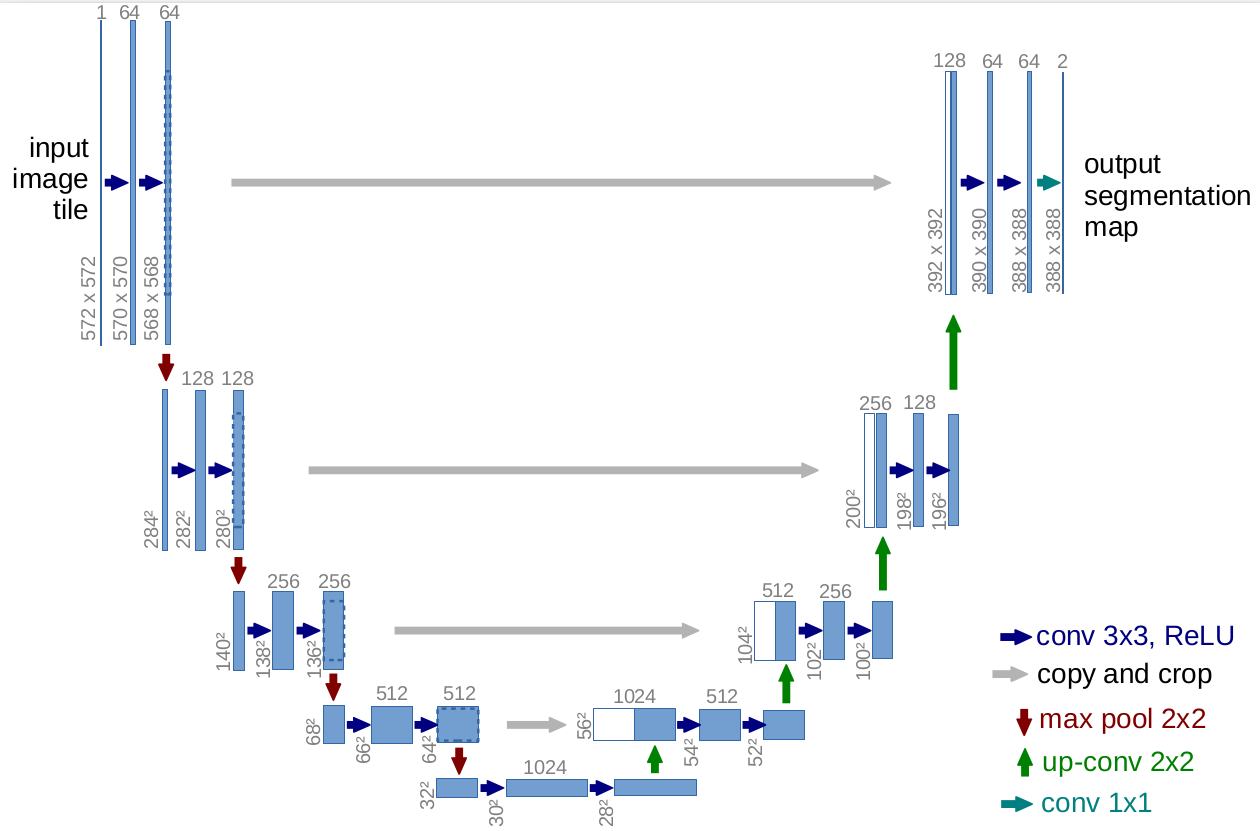
\includegraphics[width=14cm]{images/unet.png}
\caption{The U-Net architecture \cite{ronneberger2015u}.}
\label{unet}
\end{figure}

The encoder part is a standard deep convolutional neural network, doing feature detection with continuously bigger features using convolutional layers.
It can be replaced by more complex convolutional neural network architectures like ResNet \cite{he2016deep}.

The decoder part on the right side is used to actually generate the segmentation output. The max pooling in the encoder part makes the processed image continuously smaller,
to detect bigger features. The decoder does the counterpart, it increases the image until is has (almost) the same size as the input image again. It not only uses
the smallest feature map produced by the last convolutional layer of the encoder, but also the feature maps of the last convolutional layer of every encoder block.
A block contains two convolutional layers and corresponding ReLU activation functions. The upscaling from one decoder block to the next (the green arrows in the diagram) are
implemented with standard image upscaling algorithms like bilinear upsampling.

\subsection{Implementation}
There are already many implementations of the U-Net architecture for PyTorch. We decided to do an independent implementation
to understand the inner workings of the U-Net.

Two implementations on GitHub provided some ideas to enhance the implementation:

The implementation by Naoto Usuyama \cite{unetmilesial} shows the idea to use padding on the convolutional layer. This way, the size of the convolutional layers inside the same block stay the same, and no calculations for the channel sizes are necessary.

The implementation by milesial \cite{unetmilesial} introduces the possibility to use batch normalization after every convolutional layer, which increased the performance
of the network significantly (see next chapter).

